\documentclass[tikz,border=2pt]{standalone}
\usepackage{graphicx}
\usepackage{xcolor}
\usepackage[scaled=0.93]{helvet}
\renewcommand{\familydefault}{\sfdefault}

\definecolor{UTBurnt}{RGB}{191,87,0}
\definecolor{UTDark}{RGB}{51,63,72}

\begin{document}
\begin{tikzpicture}
  \node[anchor=north west,inner sep=0pt] (a) at (0,0)
    {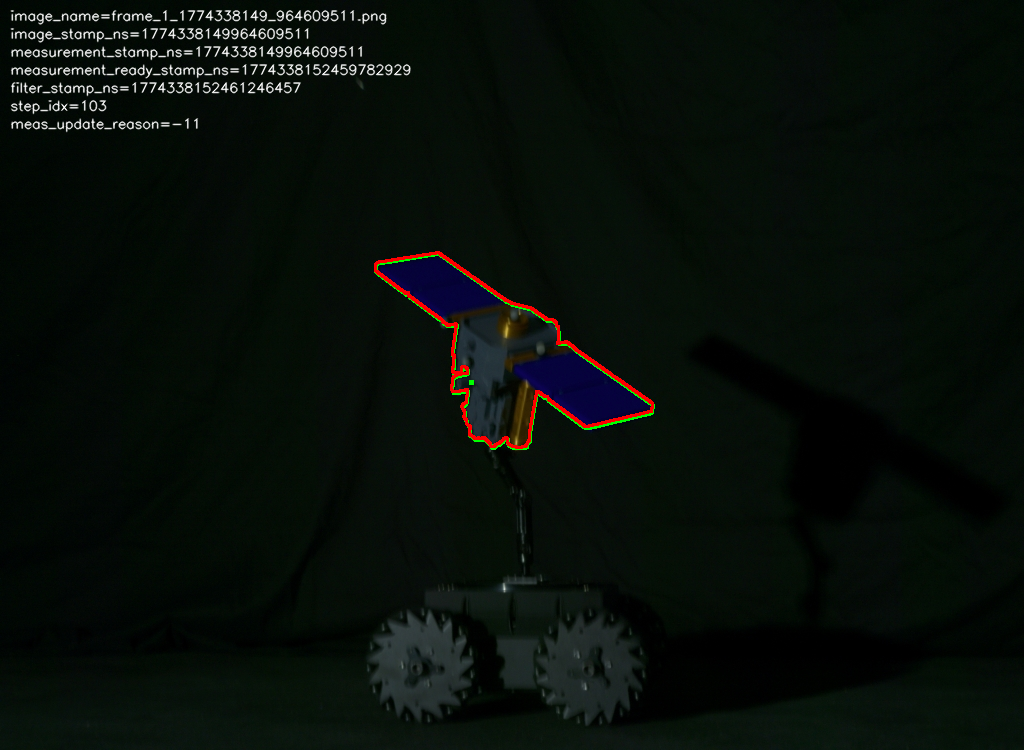
\includegraphics[width=12.6cm,trim=0 55 0 130,clip]{fig_overlay_example_1.png}};
  \node[anchor=north west,inner sep=0pt] (b) at (0,-7.05)
    {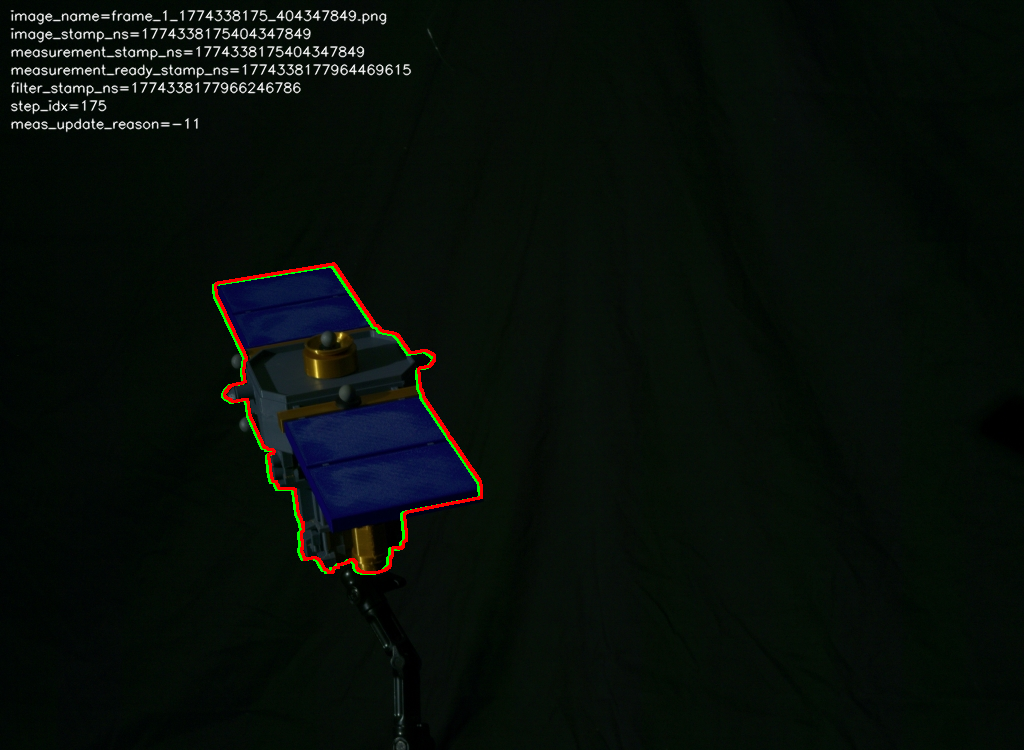
\includegraphics[width=12.6cm,trim=0 55 0 130,clip]{fig_overlay_example_2.png}};

  \draw[UTBurnt,line width=0.7pt] (0,0) rectangle (12.6,-6.96);
  \draw[UTBurnt,line width=0.7pt] (0,-7.05) rectangle (12.6,-14.01);
  \node[anchor=north west,fill=UTBurnt,text=white,font=\bfseries\scriptsize,
        inner xsep=5pt,inner ysep=2pt] at (0.10,-0.10)
    {Case A};
  \node[anchor=north west,fill=UTBurnt,text=white,font=\bfseries\scriptsize,
        inner xsep=5pt,inner ysep=2pt] at (0.10,-7.15)
    {Case B};

\end{tikzpicture}
\end{document}
